\part{Experiments}\label{chapter:experiments_and_results}
As mentioned in the previous chapter, the process of finding was an iterative one of running an experiment, analyzing the generated data, draw conclusions and then repeat the steps with a new experiments designed to amend the mistakes of the previous experiment. This chapter will go through the results that were obtained from each of the data sets. A summary and discussion of the results is found in chapter \ref{chapter:discussion}.

\section{Overview of experiments}\label{section:experiments_overview}
The model has many parameters, and doing an exhaustive search over the entire parameter space is not possible. Instead, a genetic algorithm (GA) was used to do targeted searches of the parameters. Depending on how the GA was set up, different areas of the search space was searched. Even when using a GA, some parameters had to be fixed. However, fixing parameters means that the effect of the fixed parameter on the behavior of the model remains unknown, since only a subspace of the entire parameter space is searched. For this reason the genetic algorithm was executed several times, each creating a data set containing fitness values for different parts of the parameter space. Each of these data set can be analyzed, providing information which can be corroborated in order to form an understanding of the overall market behavior.

Table \ref{table:datasets_overview} contains an overview of the different data sets, showing which parameters were fixed, and which were included as genes in the genetic algorithm.

In the following four experiments, the genetic algorithm was set to minimize all four fitness-measures.

\begin{description}
\item[\dthree: Varying the number of HFT agents, and all latency related parameters] This data set was generated by including all the model parameters concerning time latency as well as the number of agents into the individuals in the genetic algorithm. Due to the high number of variables, the data turned out to be difficult to analyze, as too many factors pertaining to the simultaneous change of several parameters influenced the fitness values.
\item[\dnine: Fixing the number of agents while varying latency parameters] The analysis of \dthree{} showed that when minimizing the four fitness-measures, the genetic algorithm tended to select  model containing few or no HFT agents. The case of a market with no market makers and no chartists can safely be said to be trivial. Hence, in experiment \dnine{}, the number of HFT agents were fixed to $\ssmmnAgents = 30$ and $\scnAgents = 100$.
\item[\dten: Fixing the number of HFT chartists] Since \dnine{} kept \ssmmnAgents{} and \scnAgents{} constant, the experiment did not reveal anything on how the market behavior changes when the number of agents changes. In order to investigate the impact of having many or few HFT market makers, \ssmmnAgents{} was varied in this experiment. Although it is also of interest how the market behavior depends on the number of HFT chartists, including \scnAgents{} as a gene would yield results similar to those obtained in \dthree. For this reason the number of HFT chartists was fixed to $\scnAgents = 150$.
\item[\deleven: Fixing the number of HFT market makers] This experiment was carried out in order to investigate the impact of the number of HFT chartists on the market behavior, and is supplementary to \dten.
\end{description}


\begin{table}
\begin{tabular}{|l|L|E|L|}
\toprule
ID & Description & Fixed parameters& As genes \\
\midrule
\dthree{} & All parameters varied& $\scordervolumemu=10$,$\scordervolumes=3$,$\ssmmordervolumemu=50$,$\ssmmordervolumes=20$,$\scticksbeforereactingmu=2$,$\scticksbeforereactings=5$,$\scpriceticksizemu=3$,$\scpriceticksizes=2$ &  \sclatencymu, \sclatencys, \scnAgents, \scthinkmu, \scthinks, \sctimehorizonmu, \sctimehorizons, \scwaitTimeBetweenTradingmu, \scwaitTimeBetweenTradings, \ssmmlatencymu, \ssmmlatencys, \ssmmnAgents, \ssmmthinkmu, \ssmmthinks\\
\midrule
\dnine & Fixed number of HFT agents &$\ssmmnAgents = 30$, $\scnAgents = 100$,$\scordervolumemu=10$,$\scordervolumes=3$,$\ssmmordervolumemu=50$,$\ssmmordervolumes=20$,$\scticksbeforereactingmu=2$,$\scticksbeforereactings=5$,$\scpriceticksizemu=3$, $\scpriceticksizes=2$ & \scthinkmu, \scthinks, \sctimehorizonmu, \sctimehorizons, \scwaitTimeBetweenTradingmu, \scwaitTimeBetweenTradings, \ssmmlatencymu, \ssmmlatencys, \ssmmnAgents, \ssmmthinkmu, \ssmmthinks \\
\midrule
\dten & Fixed number of HFT chartists and fixed strategy parameters & $\scnAgents = 150$, $\ssmmthinkmu = \scthinkmu = 50$, $\ssmmthinks = \scthinks = 20$, $\sctimehorizonmu = 5000$, $\sctimehorizons = 2000$, $\scwaitTimeBetweenTradingmu = 50$, $\scwaitTimeBetweenTradings = 20$,$\scordervolumemu=10$,$\scordervolumes=3$,$\ssmmordervolumemu=50$,$\ssmmordervolumes=20$,$\scticksbeforereactingmu=2$,$\scticksbeforereactings=5$, $\scpriceticksizemu=3$,$\scpriceticksizes=2$  & \ssmmnAgents, \sclatencymu, \sclatencys, \ssmmlatencymu, \ssmmlatencys \\
\midrule
\deleven & Fixed number of HFT market makers and fixed strategy parameters & $\ssmmnAgents = 52$, $\ssmmthinkmu = \scthinkmu = 50$, $\ssmmthinks = \scthinks = 20$, $\sctimehorizonmu = 5000$, $\sctimehorizons = 2000$, $\scwaitTimeBetweenTradingmu = 50$, $\scwaitTimeBetweenTradings = 20$,$\scordervolumemu=10$,$\scordervolumes=3$,$\ssmmordervolumemu=50$,$\ssmmordervolumes=20$,$\scticksbeforereactingmu=2$,$\scticksbeforereactings=5$, $\scpriceticksizemu=3$,$\scpriceticksizes=2$  & \ssmmnAgents, \sclatencymu, \sclatencys, \ssmmlatencymu, \ssmmlatencys \\
\bottomrule
\end{tabular}
\caption{Overview of datasets}
\label{table:datasets_overview}
\end{table}


\subsection{Correlation between fitness measures}\label{section:correlation_fitness}
A factor which influences the evolution of parameters is correlation between the fitness-measures. If two or more fitness measures have non-negative correlation coefficients, individuals will be statistically more likely to get good scores in the correlated fitness measures at the same time. Since all fitness measures are given equal weight in the selection process, individuals scoring well in the correlated fitness-measures will win over individuals which score well on another, statistically independent fitness measure. It is therefore important to compare the selection tendencies with the correlation between fitness-measures. Figure \ref{figure:fitness_correlation} shows a plot of the correlation matrix for \dten{} and \deleven. Since later generations will be affected by the biased selection and therefore contain more individuals which did well on the correlated fitness measures, the correlation coefficients in the figure were calculated over individuals in the first generation only.
\begin{figure}
	%issue 15
	\centering
	\subcaptionbox{\dten}
	[0.49\linewidth]{\includegraphics[width=0.5\textwidth]{fitness_correlation/d10/correlation_matrix.png}}
	\subcaptionbox{\deleven}
		[0.49\linewidth]{\includegraphics[width=0.5\textwidth]{fitness_correlation/d11/correlation_matrix.png}}
	\caption{Correlation between model fitness measures}
	\label{figure:fitness_correlation}
\end{figure}

For instance, the correlation between \overshoot{} and \stdev{} means that an individual which scores a good \overshoot-fitness will be statistically likely to also score a good \stdev-fitness. Since all four fitness measures are weighed evenly in the selection, models with behavior which is assigned good values for \overshoot{} and \stdev{} will score a better overall fitness than a simulation with a good \timetoreachnewfundamental-fitness. In other words, the correlation between \stdev{} and \overshoot{} means that stable individuals will outlive fast individuals as they are selected for breeding more often. This is not a property of the model itself, but something that arises due to the definition of the fitness measures. 

The correlations also speak of trade-offs between speed and stability in the model. For instance, a negative correlation between \overshoot{} and \timetoreachnewfundamental{} means that the model is statistically likely to have a large overshoot when it responds quickly to the change in the fundamental.

\section{Fitness and parameter evolution}\label{section:fitness_and_paraeter_evolution}


\subsection{Variable number of market makers}

Figure \ref{fig:d10_evolution_fitness} shows the evolution of the four fitness measures. The population wide mean is plotted along the median and minimum statistics. Since all four fitness measures were minimized, the curve for the minimum value shows the best individual alive during each generation, with respect to each fitness measure. While the mean reflects how the overall population is evolving,  the median is useful as it gives an insight into how skewed the population wide distribution of parameters is. 


\begin{figure}
	%issue 15
	\centering
	\subcaptionbox{Evolution of \roundstable\label{fig:d10_evolution_fitness_a}}
	[0.49\linewidth]{\includegraphics[width=0.5\textwidth]{82_generation_plots/d10/round_stable.png}}
	\subcaptionbox{Evolution of \timetoreachnewfundamental\label{fig:d10_evolution_fitness_b}}
	[0.49\linewidth]{\includegraphics[width=0.5\textwidth]{82_generation_plots/d10/time_to_reach_new_fundamental.png}}
	\subcaptionbox{Evolution of \stdev\label{fig:d10_evolution_fitness_c}}
	[0.49\linewidth]{\includegraphics[width=0.5\textwidth]{82_generation_plots/d10/stdev.png}}
	\subcaptionbox{Evolution of \overshoot\label{fig:d10_evolution_fitness_d}}
	[0.49\linewidth]{\includegraphics[width=0.5\textwidth]{82_generation_plots/d10/overshoot.png}}
	\caption{Evolution of the four fitness measures in experiment \dten}
	\label{fig:d10_evolution_fitness}
\end{figure}





\begin{description}
\item[Model stability]
Figure \ref{fig:d10_evolution_fitness_a}: shows that  the GA quickly manages to find some parameters which cause the simulation to stabilize quickly. However, these individuals do not manage to dominate the population evident by the mean and median curves remaining almost the same until generation 30 or so. In the next 20 generations the population undergoes a rapid change, as the population wide average of \roundstable{} drops from close to $10^5$ to around $2\cdot 10^4$ rounds on average. The disparity between the mean and the median indicates that the population undergoes a rapid change in the same period, from mostly containing unstable individuals to mostly containing stable individuals. In generation 42, the median curve crosses the mean curve, which means that the the population contain as many stable simulations as it contain unstable simulations. From that point on the unstable simulations are quickly replaced by stable individuals.
\item[Price fluctuations and overshoot]
During the same period, the population average \stdev{} also decreases fairly rapidly, but the drop is less pronounced than the drop in \stdev. As figures \ref{fig:d10_evolution_parameters_a} and \ref{fig:d10_evolution_parameters_b} show, the number of market makers rapidly increased during this period, as did the average latency of the market makers. Since the mean and median are close in both figure\footnote{Since \overshoot{} is discrete, the median and $\min$ statistics are also discrete}, the mean is representative of the evolution of the entire population.
\item[Responsiveness]
\timetoreachnewfundamental{} measures the time it takes for the model to react to the shock in the fundamental, and the evolution of the population wide statistics is shown on figure \ref{fig:d10_evolution_fitness_b}. Although the GA is instructed to minimize \timetoreachnewfundamental{} in order to look for more faster models, it clearly fails to do this. Indeed, the most responsive simulation took only about 4000 rounds to reach the new fundamental, but this individual died out in favor of slower individuals. In the last generation the most responsive simulation took around 14000 rounds to reach the new fundamental. The reasons for this failure to locate responsive models is discussed in section \ref{section:correlation_fitness}. In (the A) large change of the average of \timetoreachnewfundamental{} happens in the rounds five to 15. In this period, the median is lower than the mean, which means that the growth in the mean can be attributed to a minority of individuals.
\end{description}


On figures \ref{fig:d10_evolution_fitness} and \ref{fig:d10_evolution_parameters}, the two areas shaded in a light blue and light red respectively show the two periods during which there was a drastic change in parameters and fitness-values. By comparing the time at which parameters and fitness-values change, it is possible to get an idea of how parameters influence the fitness-values. To that end, figure \ref{fig:d10_evolution_parameters} shows the evolution of each of the parameters that were varied by the GA\footnote{Since the median was found to follow the mean nicely for all the parameters, the medians are not displayed. Also, the gray error bars show the population wide variance}.
\begin{figure}
	%issue 15
	\centering
	\subcaptionbox{Evolution of \ssmmlatencymu{} and \sclatencymu\label{fig:d10_evolution_parameters_a}}
	[0.49\linewidth]{\includegraphics[width=0.5\textwidth]{82_generation_plots/d10/latpars_mu.png}}
	\subcaptionbox{Evolution of \ssmmlatencys{} and \sclatencys\label{fig:d10_evolution_parameters_b}}
	[0.49\linewidth]{\includegraphics[width=0.5\textwidth]{82_generation_plots/d10/latpars_s.png}}
	\subcaptionbox{Evolution of \ssmmnAgents\label{fig:d10_evolution_parameters_c}}
	[0.49\linewidth]{\includegraphics[width=0.5\textwidth]{82_generation_plots/d10/nAgents.png}}
	\caption{Evolution of the model parameters in experiment \dten}
	\label{fig:d10_evolution_parameters}
\end{figure}

The two periods indicated by the shaded squares seem to reflect some sudden changes in the parameters.

\begin{description}
\item[Average agent latency]  As is shown on figure \ref{fig:d10_evolution_parameters_a}, individuals containing large latency parameters are selected for both HFT market makers and HFT chartists. $\E{\sclatencymu}$ grows grows quickly during the first 20 rounds (blue shade). Referring back to figure \ref{fig:d10_evolution_fitness}, it is seen that $\E{\timetoreachnewfundamental}$ and $\E{\overshoot}$ grows and shrinks respectively. As for $\E{\ssmmlatencymu}$, it grows from rounds 20 through 50 (red shade), and this  seems to be strongly reflected in the growth of $\E{\roundstable}$, and to a lesser degree a decline in $\E{\overshoot}$ and $\E{\stdev}$. Furthermore, the small size of the error bars on both curves show that the population consistently moves towards containing more individuals with larger latency parameters for both HFT agent types. While initially $\E{\ssmmlatencymu} \approx \E{\sclatencymu}$, the population wide mean $\E{\sclatencymu}$ ends up being roughly 1.5 times larger than $\E{\sclatencymu}$. Finally, note also that the growth of  $\E{\sclatencymu}$ and $\E{\ssmmlatencymu}$ seem to be somewhat independent, as they sometimes grow together, sometimes not.

\item[Number of market makers] The number of market makers increases almost every generation, but grows especially quickly through rounds 20 to 50 (red shade)

\item[Variance of agent latency] Figure \ref{fig:d10_evolution_parameters_b}: The trends for $\E{\sclatencys}$ and $\E{\ssmmlatencys}$ are less clear, as the population-wide variances $\Var{\sclatencymu}$ and $\Var{\ssmmlatencymu}$, illustrated by the large error bars, are high compared to the change in $\E{\sclatencymu}$ and $\E{\ssmmlatencymu}$. While this could mean that the market behaves more regularly when the difference between the latency parameters of the trading agents is smaller, further experiments would have to be carried out to confirm this fact.
\end{description}

In summary, the genetic algorithm prefers simulations with many, but relatively slow market makers. Apparently simulations with slow chartists also outperformed those with fast chartists, but since the number of HFT chartists was fixed at $\scnAgents = $, this experiment does not reveal how the simulation would perform with more (or less) chartists. It is possible to imagine that the market would perform just as well with a few and fast chartists. Later sections contain the analysis of experiment \deleven{} in which the number of chartists were varied. The discussion above can be summarized as follows:

\begin{enumerate}
\item The responsiveness of the market is influenced by latency of the chartists. Slower chartists made the market require more time to respond to the fundamental shock.
\item The time it takes for the market to adjust to the shock in the fundamental is by the number of market makers and on the latency of the market makers. More but slower market makers seems to make the market settle within the stability margin faster.
\item The overshoot, as well as the average size of the price fluctuations of the market, are both influenced by the latency of both agent types, as well as the number of market makers.
\item The market was more stable but reacted slowly when the chartists were slower than the market makers.
\end{enumerate}
The accuracy of the above analysis is limited as it only looks at population wide statistics at a given point in the duration of the GA. The following section contain an analysis in which the generation to which each data point belongs is considered irrelevant. The analysis will try to confirm each of the four statements above.

\subsection{Fixed number of chartists and market makers}

\begin{figure}
	%issue 15
	\centering
	\subcaptionbox{Evolution of \roundstable\label{fig:d9_evolution_fitness_a}}
	[0.49\linewidth]{\includegraphics[width=0.5\textwidth]{82_generation_plots/d9/round_stable.png}}
	\subcaptionbox{Evolution of \timetoreachnewfundamental\label{fig:d9_evolution_fitness_b}}
	[0.49\linewidth]{\includegraphics[width=0.5\textwidth]{82_generation_plots/d9/time_to_reach_new_fundamental.png}}
	\subcaptionbox{Evolution of \stdev\label{fig:d9_evolution_fitness_c}}
	[0.49\linewidth]{\includegraphics[width=0.5\textwidth]{82_generation_plots/d9/stdev.png}}
	\subcaptionbox{Evolution of \overshoot\label{fig:d9_evolution_fitness_d}}
	[0.49\linewidth]{\includegraphics[width=0.5\textwidth]{82_generation_plots/d9/overshoot.png}}
	\caption{Evolution of the four fitness measures in experiment \dnine}
	\label{fig:d9_evolution_fitness}
\end{figure}


\begin{figure}
	%issue 15
	\centering
	\subcaptionbox{Evolution of \ssmmlatencymu{} and \sclatencymu\label{fig:d9_evolution_parameters_a}}
	[0.49\linewidth]{\includegraphics[width=0.5\textwidth]{82_generation_plots/d9/latpars_mu.png}}
	\subcaptionbox{Evolution of \ssmmlatencys{} and \sclatencys\label{fig:d9_evolution_parameters_b}}
	[0.49\linewidth]{\includegraphics[width=0.5\textwidth]{82_generation_plots/d9/thinkpars_mu.png}}
	\subcaptionbox{Evolution of \ssmmnAgents\label{fig:d9_evolution_parameters_c}}
	[0.49\linewidth]{\includegraphics[width=0.5\textwidth]{82_generation_plots/d9/sctimehorizon_mu.png}}
	\subcaptionbox{Evolution of \ssmmnAgents\label{fig:d9_evolution_parameters_d}}
	[0.49\linewidth]{\includegraphics[width=0.5\textwidth]{82_generation_plots/d9/scwaittime_mu.png}}
	\caption{Evolution of the model parameters in experiment \dten}
	\label{fig:d9_evolution_parameters}
\end{figure}

When the GA cannot change the number of chartists and market makers, it has to find better fitness values by selecting the right latency parameters. As shown on figure \ref{fig:d9_evolution_fitness}, the GA managed to find models with little or no overshoot, non-flickering prices, and which become stable. The price of having these nice qualities seems to be a slower response time to the shock. The GA find these well-behaving markets by selecting latency parameters such that the chartists are slower than the market makers. $\E{\sctimehorizonmu}$ and $\E{\scwaitTimeBetweenTradingmu}$ change little or are more or less unchanged, which seems to indicate that they have little effect of the fitness values, at least compared to other time related parameters such as \sclatencymu, \ssmmlatencymu, \scthinkmu{} and \ssmmthinkmu. 


\subsection{Variable number of chartists}
The evolution of the fitness values in \deleven, shown in figure \ref{fig:d11_evolution_fitness} fluctuate significantly more than in \dnine{} and \dten. In contrary to the two other experiments, the GA here manages to decrease \timetoreachnewfundamental, and $\E{\timetoreachnewfundamental}$ drops almost 10000 rounds around generation 200. At the same time $\E{\overshoot}$, $\E{\stdev}$ and $\E{\roundstable}$ all rise, again indicating the there exists a trade-off between speed and stability in the model. At the point in the evolution where $\E{\timetoreachnewfundamental}$ drops, several interesting things happen with the model parameters that live in the population. First of all the number of chartists increase dramatically, again pointing towards more chartists making the markets fast and unstable. Secondly, the market maker latency also drops to around the same level as the chartist latency. This is interesting because it could mean that the faster market makers help drive the market towards a larger overshoot.

\begin{figure}
	%issue 15
	\centering
	\subcaptionbox{Evolution of \roundstable\label{fig:d11_evolution_fitness_a}}
	[0.49\linewidth]{\includegraphics[width=0.5\textwidth]{82_generation_plots/d11/round_stable.png}}
	\subcaptionbox{Evolution of \timetoreachnewfundamental\label{fig:d11_evolution_fitness_b}}
	[0.49\linewidth]{\includegraphics[width=0.5\textwidth]{82_generation_plots/d11/time_to_reach_new_fundamental.png}}
	\subcaptionbox{Evolution of \stdev\label{fig:d11_evolution_fitness_c}}
	[0.49\linewidth]{\includegraphics[width=0.5\textwidth]{82_generation_plots/d11/stdev.png}}
	\subcaptionbox{Evolution of \overshoot\label{fig:d11_evolution_fitness_d}}
	[0.49\linewidth]{\includegraphics[width=0.5\textwidth]{82_generation_plots/d11/overshoot.png}}
	\caption{Evolution of the four fitness measures in experiment \deleven}
	\label{fig:d11_evolution_fitness}
\end{figure}


\begin{figure}
	%issue 15
	\centering
	\subcaptionbox{Evolution of \ssmmlatencymu{} and \sclatencymu}
	[0.49\linewidth]{\includegraphics[width=0.5\textwidth]{82_generation_plots/d11/latpars_mu.png}}
	\subcaptionbox{Evolution of \ssmmlatencys{} and \sclatencys}
	[0.49\linewidth]{\includegraphics[width=0.5\textwidth]{82_generation_plots/d11/latpars_s.png}}
	\subcaptionbox{Evolution of \scnAgents}
	[0.49\linewidth]{\includegraphics[width=0.5\textwidth]{82_generation_plots/d11/nAgents.png}}
	\caption{Evolution of the model parameters in experiment \deleven}
	\label{fig:d11_evolution_parameters}
\end{figure}

Market makers become slower and the chartists become faster. At the same time, the number of chartists rise rapidly



\begin{itemize}
\item A high number of market makers enable the market to respond quickly to the shock, but also cause the traded price to flicker more, and for the model to have a larger overshoot.
\item Slower market makers also cause the market to respond faster to the shock
\end{itemize}


\section{Population-wide parameter/fitness correlations}
This section contains several figures which illustrate how the model fitness varies with the model parameters. In the figures showing the data from experiment \deleven, simulations with $\overshoot>10$ are removed in order to make the figures easier to interpret. In the following, the notation $\meanpopulation{\cdot}$ is used for the population wide average of a model parameter of fitness measure. For instance, $\meanpopulation{\overshoot}$ is the average market overshoot, where the average is calculated over the total population of individuals that ever lived in the genetic algorithm.

\subsection{Number of market makers}
The number of market makers was kept fixed in experiments \dnine{} and \deleven, but was varied in experiment \dten.
\begin{figure}
	%issue 15
	\centering
	\subcaptionbox{Correlation between \ssmmnAgents{} and \overshoot\label{fig:d10_parvfit_ssmmnAgents_a}}
	[0.49\linewidth]{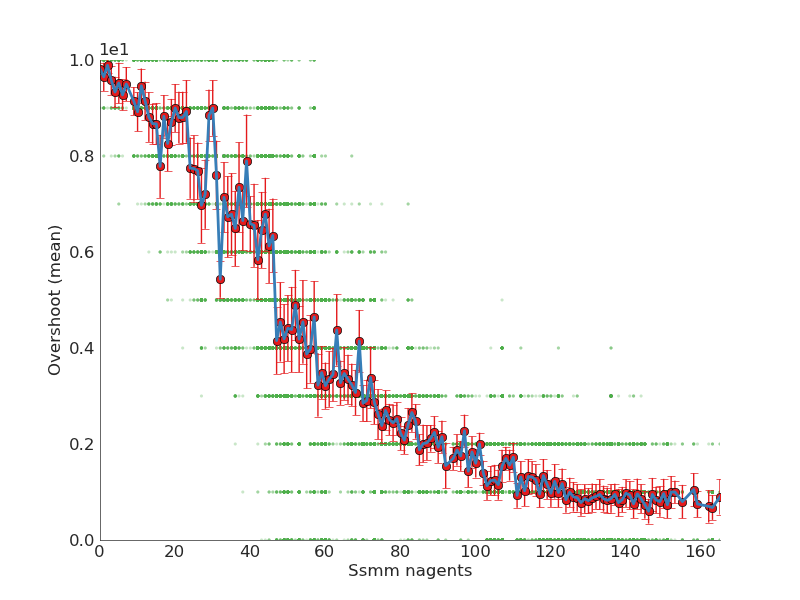
\includegraphics[width=0.5\textwidth]{101_pars_vs_fits/d10/ssmm_nAgents__vs__overshoot(mean)_scatter.png}}
	\subcaptionbox{Correlation between \ssmmnAgents{} and \roundstable\label{fig:d10_parvfit_ssmmnAgents_b}}
	[0.49\linewidth]{\includegraphics[width=0.5\textwidth]{101_pars_vs_fits/d10/ssmm_nAgents__vs__round_stable(mean)_scatter.png}}
	\subcaptionbox{Correlation between \ssmmnAgents{} and \stdev\label{fig:d10_parvfit_ssmmnAgents_c}}
	[0.49\linewidth]{\includegraphics[width=0.5\textwidth]{101_pars_vs_fits/d10/ssmm_nAgents__vs__stdev(mean)_scatter.png}}
	\subcaptionbox{Correlation between \ssmmnAgents{} and \timetoreachnewfundamental\label{fig:d10_parvfit_ssmmnAgents_d}}
	[0.49\linewidth]{\includegraphics[width=0.5\textwidth]{101_pars_vs_fits/d10/ssmm_nAgents__vs__time_to_reach_new_fundamental(mean)_scatter.png}}
	\caption{Correlation between \ssmmnAgents{} and the four fitness measures in experiment \dten}
	\label{fig:d10_parvfit_ssmmnAgents}
\end{figure}
Figure \ref{fig:d10_parvfit_ssmmnAgents} shows how the number of market makers correlates with the model fitness in experiment \dten. Evidently a large number of market makers reduces the overshoot, whereas the market virtually always have an overshoot when there are few or no market makers. The same is true for the trade prices flicker: few market makers always means flickering prices. A higher number of market makers cause the market to be less responsive, while fewer market makers have the opposite effect. Finally, the number of market makers also influences how quickly the market settles within the stability margin, as markets with more market makers become stable faster than markets with few agents. Table \ref{table:ssmmnagents_quantiles} shows the average fitness values for models where the number of market maker agents was respectively below and above the first ($q_{1}$) and ninth ($q_{9}$) 10-quantiles in the dataset.  The two quantiles were at $q_{1} =46 $ and $q_{9} = 136$. It is seen that the market containing a large number of market makers (more than 136) had a much smaller overshoot, less flickering prices, a slower response time, and stayed within the stability margin faster, compared to the markets with a low (less than 46) number of market makers.

\begin{table}
\centering
\begin{tabular}{lrr}
\toprule
\dten &       $\ssmmnAgents < q_{1}$ &       $\ssmmnAgents > q_{9}$ \\
\midrule
\overshoot                     &     7.5 &     0.8 \\
\roundstable                  & 89876.2 & 18546.9 \\
\stdev              &     1.6 &     0.6 \\
\timetoreachnewfundamental & 12590.5 & 19832.1 \\
\bottomrule
\end{tabular}
\caption{Average fitness values for the market with the top 10\% highest and 10\% lowest number of market makers}
\label{table:ssmmnagents_quantiles}
\end{table}




\subsection{Market maker latency}
The parameters controlling the market maker latency was varied in experiments \dnine, \dten{} and \deleven. However, since the data from \dnine{} turned out to be too noisy due to the large number of parameters included in the search, only data from \dten{} and \deleven{} was used. 

\subsubsection*{Fixing the number of chartists}
In experiment \dten, the number of chartists was kept fixed at $\scnAgents = 150$, while \ssmmnAgents{} was varied by the GA. In this case, the \ssmmlatencymu{} is found to be somewhat correlated with the fitness measures as illustrated on figure \ref{fig:d10_parvfit_ssmmlatencymu}. Especially for $\ssmmlatencymu > 50$, the data seems to be consistent, as the error bars showing the standard deviation of the data are small in this region. However, for $\ssmmlatencymu < 50$, the model behavior is no longer predictable by using \ssmmlatencymu{} alone. Figure \ref{fig:faster_mm_makes_worse_markets/d10/MM_mmlatency} shows line plots of the four fitness measures plotted against \ssmmlatencymu. Each line shows the average fitness of markets in which the number of market makers is in a limited range as shown in the legend. The figure shows that even though the market maker latency does influence the market, the effect is secondary to that of the number of agents. For instance, when the market contains less than 25 market makers, all four fitness measures are more or less unchanged, as is evident by the nearly flat red curves. As the number of market makers grow, so does the importance of how fast they are. The average overshoot and the average time to catch up to the new fundamental only change slightly, even with over 100 market makers (yellow line). On the other hand, the average price flickering and the average number of rounds it takes for the market to settle within the stability margin both change significantly with the market maker speed for $\ssmmnAgents > 50$. In summary, figure \ref{fig:faster_mm_makes_worse_markets/d10/MM_mmlatency} shows that in a market with only a few market makers, these agents have little influence no matter how fast they are. As the number of market makers grow, so does the collective force of all the market makers, and so does the importance of how slow or fast these agents are. 
\begin{figure}
	%issue 15
	\centering
	\subcaptionbox{Correlation between \ssmmlatencymu and \overshoot\label{fig:d10_parvfit_ssmmlatencymu_a}}
	[0.49\linewidth]{\includegraphics[width=0.5\textwidth]{101_pars_vs_fits/d10/ssmm_latency_mu__vs__overshoot(mean)_scatter.png}}
	\subcaptionbox{Correlation between \ssmmlatencymu and \roundstable\label{fig:d10_parvfit_ssmmlatencymu_b}}
	[0.49\linewidth]{\includegraphics[width=0.5\textwidth]{101_pars_vs_fits/d10/ssmm_latency_mu__vs__round_stable(mean)_scatter.png}}
	\subcaptionbox{Correlation between \ssmmlatencymu and \stdev\label{fig:d10_parvfit_ssmmlatencymu_c}}
	[0.49\linewidth]{\includegraphics[width=0.5\textwidth]{101_pars_vs_fits/d10/ssmm_latency_mu__vs__stdev(mean)_scatter.png}}
	\subcaptionbox{Correlation between \ssmmlatencymu and \timetoreachnewfundamental\label{fig:d10_parvfit_ssmmlatencymu_d}}
	[0.49\linewidth]{\includegraphics[width=0.5\textwidth]{101_pars_vs_fits/d10/ssmm_latency_mu__vs__time_to_reach_new_fundamental(mean)_scatter.png}}
	\caption{Correlation between \ssmmlatencymu{} and fitness values (fixed \scnAgents, variable \ssmmnAgents)}
	\label{fig:d10_parvfit_ssmmlatencymu}
\end{figure}
Although the influence of $\ssmmlatencymu$ depends on $\ssmmnAgents$, 
. $q_{1}$ and $q_{1}$ 
\begin{table}
\centering
\begin{tabular}{lrr}
\toprule
\dten &       $\ssmmlatencymu < q_{1}$ &       $\ssmmlatencymu > q_{9}$ \\
\midrule
\overshoot                     &     5.6 &     0.9 \\
\roundstable                  & 85927.9 & 18329.3 \\
\stdev                         &     1.4 &     0.6 \\
\timetoreachnewfundamental & 16649.4 & 18795.3 \\
\bottomrule
\end{tabular}
\hspace*{0.4in}
\begin{tabular}{lrr}
\toprule
\deleven &       $\ssmmlatencymu < q_{1}$ &       $\ssmmlatencymu > q_{9}$ \\
\midrule
\overshoot                     &    14.2 &     1.7 \\
\roundstable                  & 81379.2 & 26153.0 \\
\stdev                         &     3.6 &     1.0 \\
\timetoreachnewfundamental & 15856.2 & 18107.4 \\
\bottomrule
\end{tabular}
\caption{Average fitness values for the market with the top 10\% highest and 10\% lowest number of market makers}
\label{table:ssmmlatencymu_quantiles}
\end{table}


The next section will examine how the market behaves with respect to how many chartists are active in the market, and with respect to the latency of the chartists.

\begin{figure}
	%issue 15
	\centering
	\subcaptionbox{\label{fig:faster_mm_makes_worse_markets/d10/overshoot_MM_mmlatency}}
	[0.49\linewidth]{\includegraphics[width=0.5\textwidth]{faster_mm_makes_worse_markets/d10/overshoot_MM_mmlatency.png}}
	\subcaptionbox{\label{fig:faster_mm_makes_worse_markets/d10/round_stable_MM_mmlatency}}
	[0.49\linewidth]{\includegraphics[width=0.5\textwidth]{faster_mm_makes_worse_markets/d10/round_stable_MM_mmlatency.png}}
	\subcaptionbox{\label{fig:faster_mm_makes_worse_markets/d10/stdev_MM_mmlatency}}
	[0.49\linewidth]{\includegraphics[width=0.5\textwidth]{faster_mm_makes_worse_markets/d10/stdev_MM_mmlatency.png}}
	\subcaptionbox{\label{fig:faster_mm_makes_worse_markets/d10/time_to_reach_new_fundamental_MM_mmlatency}}
	[0.49\linewidth]{\includegraphics[width=0.5\textwidth]{faster_mm_makes_worse_markets/d10/time_to_reach_new_fundamental_MM_mmlatency.png}}
	\caption{Relation between \ssmmnAgents, \ssmmlatencymu, and the model fitness when the number of chartists was fixed to $\scnAgents = 150$ agents. Due to missing data, some of the curves are not complete.}
	\label{fig:faster_mm_makes_worse_markets/d10/MM_mmlatency}
\end{figure}




\subsubsection{Fixing the number of market makers}
In experiment \deleven, the number of chartists was varied, while the number of market makers were kept at a constant $\ssmmnAgents = 52$ agents. While it was fairly obvious that the market would not be impacted by changing \ssmmlatencymu when only a few market makers were active, it is less obvious that the same is true for the number of chartists. Yet figure 

\begin{figure}
	%issue 15
	\centering
	\subcaptionbox{Correlation between \ssmmlatencymu and \overshoot\label{fig:d11_parvfit_ssmmlatencymu_a}}
	[0.49\linewidth]{\includegraphics[width=0.5\textwidth]{101_pars_vs_fits/d11/ssmm_latency_mu__vs__overshoot(mean)_scatter.png}}
	\subcaptionbox{Correlation between \ssmmlatencymu and \roundstable\label{fig:d11_parvfit_ssmmlatencymu_b}}
	[0.49\linewidth]{\includegraphics[width=0.5\textwidth]{101_pars_vs_fits/d11/ssmm_latency_mu__vs__round_stable(mean)_scatter.png}}
	\subcaptionbox{Correlation between \ssmmlatencymu and \stdev\label{fig:d11_parvfit_ssmmlatencymu_c}}
	[0.49\linewidth]{\includegraphics[width=0.5\textwidth]{101_pars_vs_fits/d11/ssmm_latency_mu__vs__stdev(mean)_scatter.png}}
	\subcaptionbox{Correlation between \ssmmlatencymu and \timetoreachnewfundamental\label{fig:d11_parvfit_ssmmlatencymu_d}}
	[0.49\linewidth]{\includegraphics[width=0.5\textwidth]{101_pars_vs_fits/d11/ssmm_latency_mu__vs__time_to_reach_new_fundamental(mean)_scatter.png}}
	\caption{Correlation between \ssmmlatencymu{} and fitness values (fixed \ssmmnAgents, variable \scnAgents)}
	\label{fig:d11_parvfit_ssmmlatencymu}
\end{figure}


\begin{figure}
     %issue 15
     \centering
     \subcaptionbox{}
     [0.49\linewidth]{\includegraphics[width=0.5\textwidth]{faster_mm_makes_worse_markets/d11/overshoot_SC_mmlatency.png}}
     \subcaptionbox{}
     [0.49\linewidth]{\includegraphics[width=0.5\textwidth]{faster_mm_makes_worse_markets/d11/round_stable_SC_mmlatency.png}}
     \subcaptionbox{}
     [0.49\linewidth]{\includegraphics[width=0.5\textwidth]{faster_mm_makes_worse_markets/d11/stdev_SC_mmlatency.png}}
     \subcaptionbox{}
     [0.49\linewidth]{\includegraphics[width=0.5\textwidth]{faster_mm_makes_worse_markets/d11/time_to_reach_new_fundamental_SC_mmlatency.png}}
     \caption{Relation between \ssmmnAgents, \ssmmlatencymu, and the model fitness when the number of market makers was fixed to $\ssmmnAgents = 52$ agents.}
     \label{fig:faster_mm_makes_worse_markets/d11/SC_mmlatency}
\end{figure}


\subsection{Number of chartists}
\begin{figure}
	%issue 15
	\centering
	\subcaptionbox{Correlation between \scnAgents and \overshoot\label{fig:d11_parvfit_scnagents_a}}
	[0.49\linewidth]{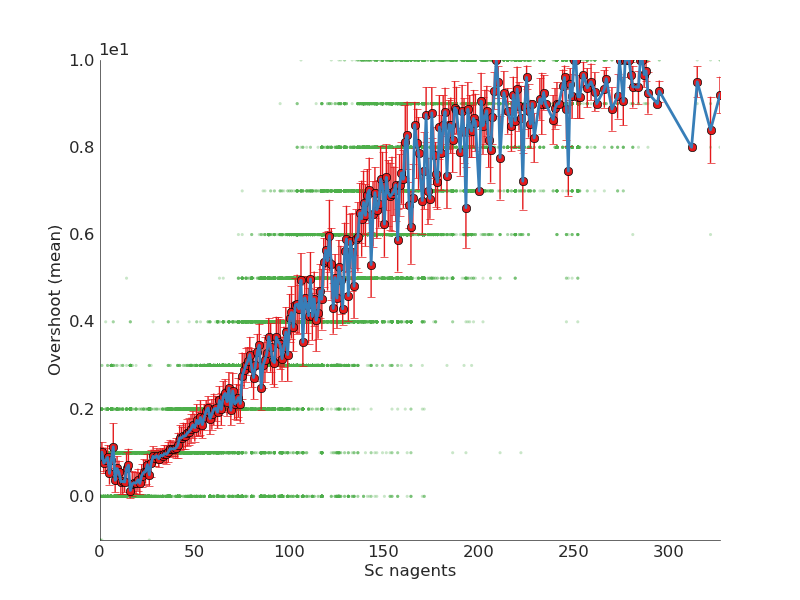
\includegraphics[width=0.5\textwidth]{101_pars_vs_fits/d11/sc_nAgents__vs__overshoot(mean)_scatter.png}}
	\subcaptionbox{Correlation between \scnAgents and \roundstable\label{fig:d11_parvfit_scnagents_b}}
	[0.49\linewidth]{\includegraphics[width=0.5\textwidth]{101_pars_vs_fits/d11/sc_nAgents__vs__round_stable(mean)_scatter.png}}
	\subcaptionbox{Correlation between \scnAgents and \stdev\label{fig:d11_parvfit_scnagents_c}}
	[0.49\linewidth]{\includegraphics[width=0.5\textwidth]{101_pars_vs_fits/d11/sc_nAgents__vs__stdev(mean)_scatter.png}}
	\subcaptionbox{Correlation between \scnAgents and \timetoreachnewfundamental\label{fig:d11_parvfit_scnagents_d}}
	[0.49\linewidth]{\includegraphics[width=0.5\textwidth]{101_pars_vs_fits/d11/sc_nAgents__vs__time_to_reach_new_fundamental(mean)_scatter.png}}
	\caption{Correlation between \scnAgents and the four fitness measures when $\ssmmnAgents = 52$ (experiment \deleven)}
	\label{fig:d11_parvfit_scnagents}
\end{figure}
Figure \ref{fig:d11_parvfit_scnagents} shows the average population wide number of agents $\E{\scnAgents}$ plotted against each of the four fitness measures, and the figures are summarized below.

\begin{itemize}
\item The more chartists a market has, the faster it responds to the fundamental. This is especially true when comparing markets with less than 100 chartists, and less pronounced when comparing markets with over 100 chartists.
\item The model overshoot is also correlated with the number of chartists in such a way that markets with more chartists have a larger overshoot on average. Whereas the market only seemed to benefit from a decreased response time when the number of chartists were kept below 100, the overshoot continues to grow steadily larger even as the number of chartists is increased beyond 100 agents.
\item \stdev{} is correlated with the number of chartists in the same way as \overshoot, such that more chartists make the traded prices flicker more.
\item Finally, the graph for \roundstable{} show that the market rarely becomes stable when it contains more than 50 chartists or so.
\end{itemize}
The large errorbars around the points with a large value of \scnAgents{} is caused by data sparsity in this region. The GA was set to search for stable markets, and since markets with a large number of chartists tend to be unstable, such markets were rarely selected for creating offspring. 





\subsection{Chartist latency}

\subsubsection*{Fixed number of chartists}

Figure \ref{fig:d10_parvfit_sclatencymu_a} shows that \sclatencymu{} is negatively correlated with \overshoot, such that markets with faster chartists are more likely to have a larger overshoot.  Next, figure \ref{fig:d10_parvfit_sclatencymu}  shows that \sclatencymu{} is negatively correlated with \stdev, such that markets with faster chartists are more likely to have flickering trade prices. 

As for the market responsiveness, it is seen that \sclatencymu{} is positively correlated with \timetoreachnewfundamental, such that markets with faster agents is more likely to have a shorter response time to the market. Figure \ref{fig:d10_parvfit_sclatencymu_d} confirms that markets with fast chartists did actually manage to reach the new fundamental price faster than those markets having slow chartists. The average response time of markets in which the chartists had a latency of less than 30 rounds was around 18000 rounds, whereas it was around 25000 rounds with chartists with more than 100 rounds of latency. The market response time is most sensitive in the range $20< \sclatencymu< 60$, and does not change much for larger latencies. 

The plots of \overshoot, \stdev{} and \timetoreachnewfundamental{} show that predicting the three fitness measures in markets with slow chartists would be more accurate than for markets with fast chartists, as the correlation of \overshoot, \stdev{} and \timetoreachnewfundamental{} with \sclatencymu{} is stronger for larger values of \sclatencymu. 

Figure \ref{fig:d10_parvfit_sclatencymu_b} shows that \sclatencymu{} is positively correlated with \roundstable, but also that the relationship between \sclatencymu{} and \roundstable{} seems highly non-linear. The figure illustrates the binary nature of the stability criteria, that is, that a simulation is either stable or not stable. This causes \roundstable{} to have a high conditional variance of \roundstable{} given \sclatencymu{} in the region $50 < \sclatencymu < 120$, meaning that that prediction of \roundstable{} from \sclatencymu{} in this region would not be very accurate. What this means is that the stability of a simulation is highly dependent on factors other than \sclatencymu, when the parameter is within 50 to 120 rounds. When the chartists are faster than 50 rounds, the market is almost always unstable, and when the chartists are slower than 120 rounds the market is almost always stable. 

\begin{figure}
	%issue 15
	\centering
	\subcaptionbox{Correlation between \sclatencymu and \overshoot\label{fig:d10_parvfit_sclatencymu_a}}
	[0.49\linewidth]{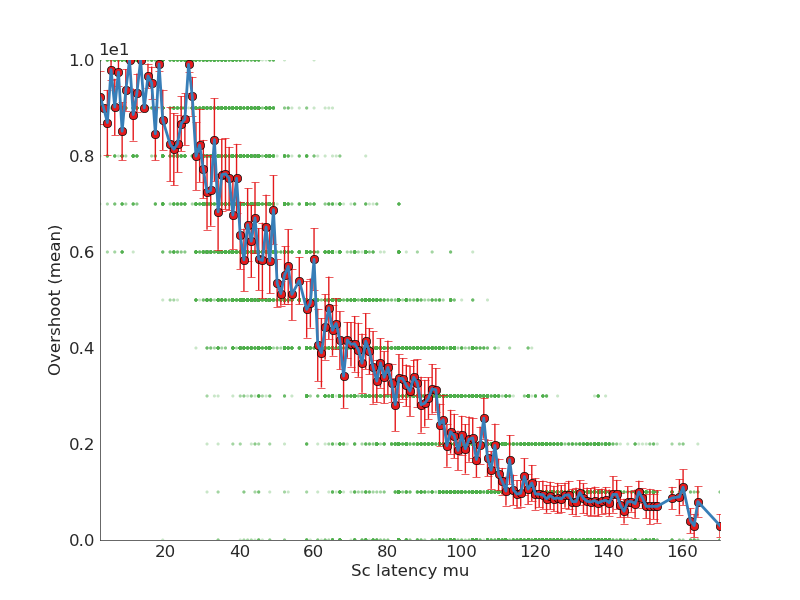
\includegraphics[width=0.5\textwidth]{101_pars_vs_fits/d10/sc_latency_mu__vs__overshoot(mean)_scatter.png}}
	\subcaptionbox{Correlation between \sclatencymu and \roundstable\label{fig:d10_parvfit_sclatencymu_b}}
	[0.49\linewidth]{\includegraphics[width=0.5\textwidth]{101_pars_vs_fits/d10/sc_latency_mu__vs__round_stable(mean)_scatter.png}}
	\subcaptionbox{Correlation between \sclatencymu and \stdev\label{fig:d10_parvfit_sclatencymu_c}}
	[0.49\linewidth]{\includegraphics[width=0.5\textwidth]{101_pars_vs_fits/d10/sc_latency_mu__vs__stdev(mean)_scatter.png}}
	\subcaptionbox{Correlation between \sclatencymu and \timetoreachnewfundamental\label{fig:d10_parvfit_sclatencymu_d}}
	[0.49\linewidth]{\includegraphics[width=0.5\textwidth]{101_pars_vs_fits/d10/sc_latency_mu__vs__time_to_reach_new_fundamental(mean)_scatter.png}}
	\caption{Correlation between chartist latency and fitness values (fixed \scnAgents, variable \ssmmnAgents)}
	\label{fig:d10_parvfit_sclatencymu}
\end{figure}

\begin{figure}
	%issue 15
	\centering
	\subcaptionbox{\label{fig:faster_mm_makes_worse_markets/d10/overshoot_MM_sclatency}}
	[0.49\linewidth]{\includegraphics[width=0.5\textwidth]{faster_mm_makes_worse_markets/d10/overshoot_MM_sclatency.png}}
	\subcaptionbox{\label{fig:faster_mm_makes_worse_markets/d10/round_stable_MM_sclatency}}
	[0.49\linewidth]{\includegraphics[width=0.5\textwidth]{faster_mm_makes_worse_markets/d10/round_stable_MM_sclatency.png}}
	\subcaptionbox{\label{fig:faster_mm_makes_worse_markets/d10/stdev_MM_sclatency}}
	[0.49\linewidth]{\includegraphics[width=0.5\textwidth]{faster_mm_makes_worse_markets/d10/stdev_MM_sclatency.png}}
	\subcaptionbox{\label{fig:faster_mm_makes_worse_markets/d10/time_to_reach_new_fundamental_MM_sclatency}}
	[0.49\linewidth]{\includegraphics[width=0.5\textwidth]{faster_mm_makes_worse_markets/d10/time_to_reach_new_fundamental_MM_sclatency.png}}
	\caption{Relation between \ssmmnAgents, \sclatencymu, and the model fitness when the number of chartists was fixed to $\scnAgents = 150 agents$. Due to missing data, some of the curves are not complete.}
	\label{fig:faster_mm_makes_worse_markets/d10/MM_sclatency}
\end{figure}




\subsubsection*{Fixed number of market makers}

\begin{figure}
	%issue 15
	\centering
	\subcaptionbox{Correlation between \sclatencymu and \overshoot\label{fig:d11_parvfit_sclatencymu_a}}
	[0.49\linewidth]{\includegraphics[width=0.5\textwidth]{101_pars_vs_fits/d11/sc_latency_mu__vs__overshoot(mean)_scatter.png}}
	\subcaptionbox{Correlation between \sclatencymu and \roundstable\label{fig:d11_parvfit_sclatencymu_b}}
	[0.49\linewidth]{\includegraphics[width=0.5\textwidth]{101_pars_vs_fits/d11/sc_latency_mu__vs__round_stable(mean)_scatter.png}}
	\subcaptionbox{Correlation between \sclatencymu and \stdev\label{fig:d11_parvfit_sclatencymu_c}}
	[0.49\linewidth]{\includegraphics[width=0.5\textwidth]{101_pars_vs_fits/d11/sc_latency_mu__vs__stdev(mean)_scatter.png}}
	\subcaptionbox{Correlation between \sclatencymu and \timetoreachnewfundamental\label{fig:d11_parvfit_sclatencymu_d}}
	[0.49\linewidth]{\includegraphics[width=0.5\textwidth]{101_pars_vs_fits/d11/sc_latency_mu__vs__time_to_reach_new_fundamental(mean)_scatter.png}}
	\caption{Correlation between chartist latency and fitness values (fixed \ssmmnAgents, variable \scnAgents)}
	\label{fig:d11_parvfit_sclatencymu}
\end{figure}

\begin{figure}
     %issue 15
     \centering
     \subcaptionbox{}
     [0.49\linewidth]{\includegraphics[width=0.5\textwidth]{faster_mm_makes_worse_markets/d11/overshoot_SC_sclatency.png}}
     \subcaptionbox{}
     [0.49\linewidth]{\includegraphics[width=0.5\textwidth]{faster_mm_makes_worse_markets/d11/round_stable_SC_sclatency.png}}
     \subcaptionbox{}
     [0.49\linewidth]{\includegraphics[width=0.5\textwidth]{faster_mm_makes_worse_markets/d11/stdev_SC_sclatency.png}}
     \subcaptionbox{}
     [0.49\linewidth]{\includegraphics[width=0.5\textwidth]{faster_mm_makes_worse_markets/d11/time_to_reach_new_fundamental_SC_sclatency.png}}
     \caption{Relation between \scnAgents, \sclatencymu, and the model fitness when the number of market makers was fixed to $\ssmmnAgents = 52$ agents.}
     \label{fig:faster_mm_makes_worse_markets/d11/SC_sclatency}
\end{figure}

Figures \ref{fig:d11_parvfit_sclatencymu} seems to indicate that no correlations exist between the speed of the chartist agents, and the model fitness measures. However, since figure \ref{fig:d10_parvfit_sclatencymu} does point towards the existence of such correlations, something else must be obscuring the scatter plots in \ref{fig:d11_parvfit_sclatencymu}. The reason is found to be that the number of chartists was not kept constant in experiment \deleven. It turns out that \sclatencymu{} is in fact correlated with \overshoot, \stdev and \timetoreachnewfundamental, but that the correlation depends heavily on the number of chartists in the market. 






\subsection{Chartist to market maker ratio}

The above observations about how the number of agents influence the stability and speed of the market pointed out that more market makers made the market slow but stable, while more chartists made the market fast, but unstable. By merging \datamatrixpar{\dten} and \datamatrixpar{\deleven}, we can calculate the ratio, \ratioagents, between the number of chartists and the number of market makers, and see how the fitness values correlate. Figure \ref{fig:parvfit_ratio_d10} and \ref{fig:parvfit_ratio_d11} show the resulting scatter plots for \dten{} and \deleven. 

\begin{figure}
	%issue 15
	\centering
	\subcaptionbox{}
	[0.49\linewidth]{\includegraphics[width=0.5\textwidth]{101_pars_vs_fits/d10/chartist_per_market_maker__vs__overshoot(mean)_scatter.png}}
	\subcaptionbox{}
	[0.49\linewidth]{\includegraphics[width=0.5\textwidth]{101_pars_vs_fits/d10/chartist_per_market_maker__vs__round_stable(mean)_scatter.png}}
	\subcaptionbox{}
	[0.49\linewidth]{\includegraphics[width=0.5\textwidth]{101_pars_vs_fits/d10/chartist_per_market_maker__vs__stdev(mean)_scatter.png}}
	\subcaptionbox{}
	[0.49\linewidth]{\includegraphics[width=0.5\textwidth]{101_pars_vs_fits/d10/chartist_per_market_maker__vs__time_to_reach_new_fundamental(mean)_scatter.png}}
	\caption{Correlations between \ratioagents{} and the fitness values when $\scnAgents = 150$}
	\label{fig:parvfit_ratio_d10}
\end{figure}

\begin{figure}
	%issue 15
	\centering
	\subcaptionbox{}
	[0.49\linewidth]{\includegraphics[width=0.5\textwidth]{101_pars_vs_fits/d11/chartist_per_market_maker__vs__overshoot(mean)_scatter.png}}
	\subcaptionbox{}
	[0.49\linewidth]{\includegraphics[width=0.5\textwidth]{101_pars_vs_fits/d11/chartist_per_market_maker__vs__round_stable(mean)_scatter.png}}
	\subcaptionbox{}
	[0.49\linewidth]{\includegraphics[width=0.5\textwidth]{101_pars_vs_fits/d11/chartist_per_market_maker__vs__stdev(mean)_scatter.png}}
	\subcaptionbox{}
	[0.49\linewidth]{\includegraphics[width=0.5\textwidth]{101_pars_vs_fits/d11/chartist_per_market_maker__vs__time_to_reach_new_fundamental(mean)_scatter.png}}
	\caption{Correlations between \ratioagents{} and the fitness values when $\ssmmnAgents = 52$}
	\label{fig:parvfit_ratio_d11}
\end{figure}








\section{Grouping models by behavior}
This section is be concerned with trying to tie various patterns of model behavior to different regions in the parameter space. The quickest way to get an idea of how the data generated by the simulations is distributed is to make scatter plots. Scatter plots are probably among the most rudimentary of techniques for data analysis, yet they can be incredibly informative, especially when the data that is visualized is low-dimensional. The data of the model fitness is four-dimensional, requiring twelve plots to visualize all combinations. However, since \overshoot is discrete with a small range of values, it is not suitable for a scatter plot. Furthermore, some scatter plots are not useful for interpretation if they do not show any structure in the data. Figure \ref{figure:d9_scatter_fitness} shows three scatter plots which were found to best illustrate the structure of the dataset from \dnine. Note also that coloring each point corresponding to its value in one dimension makes it possible to show how the data is distributed in three dimensions.
\begin{figure}
\centering
\subcaptionbox{$\log \stdev$ vs. $\log \roundstable$ vs. \timetoreachnewfundamental}
[0.49\linewidth]{\includegraphics[width=0.5\textwidth]{21_scatter_plots/d9/d.png}}
\subcaptionbox{\roundstable vs. \timetoreachnewfundamental vs. \stdev}
[0.49\linewidth]{\includegraphics[width=0.5\textwidth]{21_scatter_plots/d9/c.png}}
\subcaptionbox{$\log \overshoot$ vs . $\log \stdev$ vs. \timetoreachnewfundamental}
[0.49\linewidth]{\includegraphics[width=0.5\textwidth]{21_scatter_plots/d9/b.png}}
\caption{Scatter plots of fitness measures in experiment \dnine.}
\label{figure:d9_scatter_fitness}
\end{figure}
The scatter plots do seem to reveal some structure, the presence of large values in the \stdev feature obscures the nature of this structure, in spite of the logarithmic scaling. The plot showing $\log \stdev$ vs. $\log \roundstable$ is squeezed to the left, and the color grading on the scatter plot for $\log \overshoot$ vs . $\log \stdev$ reveals no variety in the \stdev feature. In an attempt to get some more information out of the scatter plot, data points with an overshoot of over 100 \% of the shock to the fundamental (corresponding to $\overshoot > 10$ ) are removed. The resulting scatter plots for the reduced data set are shown on figures \ref{figure:scatter_fitness_inliers_a} and \ref{figure:scatter_fitness_inliers_b}.

First of all, it is seen that while the data is distributed similarly in the three data sets, there are some differences. The data from \dnine{} seems to have many ``lonely'' data points, which are not part of any cluster, whereas the data from \dten{} somehow seems to be the cleanest of the three. In all three data sets, there are clusters of data. The clusters do not necessarily mean anything in themselves. They might simply be due to the way that data points are mutated and crossed by the GA. However, by considering which regions of the fitness space that each cluster covers, it is possible to add meaning to the clusters in terms of model behavior.

\begin{figure}
\centering
\subcaptionbox{Experiment \dnine}[0.49\linewidth]{\includegraphics[width=0.5\textwidth]{103_scatter_manual_outlier/d9/f.png}}
\subcaptionbox{Experiment \dnine}[0.49\linewidth]{\includegraphics[width=0.5\textwidth]{103_scatter_manual_outlier/d9/j.png}}
\subcaptionbox{Experiment \dten}[0.49\linewidth]{\includegraphics[width=0.5\textwidth]{103_scatter_manual_outlier/d10/f.png}}
\subcaptionbox{Experiment \dten}[0.49\linewidth]{\includegraphics[width=0.5\textwidth]{103_scatter_manual_outlier/d10/j.png}}
\subcaptionbox{Experiment \deleven}[0.49\linewidth]{\includegraphics[width=0.5\textwidth]{103_scatter_manual_outlier/d11/f.png}}
\subcaptionbox{Experiment \deleven}[0.49\linewidth]{\includegraphics[width=0.5\textwidth]{103_scatter_manual_outlier/d11/j.png}}
\caption{Scatter plot of \roundstable{} against \timetoreachnewfundamental{} with coloring showing $\log \stdev$ and \overshoot}
\label{figure:scatter_fitness_inliers_a}
\end{figure}

\begin{figure}
\centering
\subcaptionbox{Experiment \dnine}[0.49\linewidth]{\includegraphics[width=0.5\textwidth]{103_scatter_manual_outlier/d9/h.png}}
\subcaptionbox{Experiment \dnine}[0.49\linewidth]{\includegraphics[width=0.5\textwidth]{103_scatter_manual_outlier/d9/k.png}}
\subcaptionbox{Experiment \dten}[0.49\linewidth]{\includegraphics[width=0.5\textwidth]{103_scatter_manual_outlier/d10/h.png}}
\subcaptionbox{Experiment \dten}[0.49\linewidth]{\includegraphics[width=0.5\textwidth]{103_scatter_manual_outlier/d10/k.png}}
\subcaptionbox{Experiment \deleven}[0.49\linewidth]{\includegraphics[width=0.5\textwidth]{103_scatter_manual_outlier/d11/h.png}}
\subcaptionbox{Experiment \deleven}[0.49\linewidth]{\includegraphics[width=0.5\textwidth]{103_scatter_manual_outlier/d11/k.png}}
\caption{Scatter plot of $\log \stdev$ against \timetoreachnewfundamental{} with coloring showing $\roundstable$ and \overshoot}
\label{figure:scatter_fitness_inliers_b}
\end{figure}



\subsection{Manually grouping simulations by behavior}\label{section:manually_grouping_simulations}
Table \ref{table:manual_filtering} contains an overview of the named criteria used for roughly grouping simulations into different types of behavior. The following text contains the reasoning for why each of these groups are interesting.

In figure \ref{figure:scatter_fitness_inliers_a}, the black dashed lines at $\timetoreachnewfundamental = \roundstable$ divide each plot into region A, (upper left triangle) and region B (lower right triangle). Region A contains the fitness-points of the simulations which are counted as stable \textit{after} they reach the new fundamental, and region B contain those that become stable before. 

The description below provides a brief summary of which simulations belong in the two regions.
\begin{description}
\item[$\roundstable < \timetoreachnewfundamental$] This happens when the traded price never leaves the stability margin after reaching the new fundamental price. Note however that this case does not necessarily mean that the prices do not flicker. 
\item[$\roundstable > \timetoreachnewfundamental$] This happens when the traded price leaves the stability margin once or more after reaching the new fundamental. The traded price can be close to the fundamental, but flickers in and out of the stability margin as on figure \ref{figure:typical_fitness_cases}. The figure shows one example where the trade price fairly stable and with no overshoot, leading to good (low) \stdev{} and \overshoot{} fitness values to be assigned to the parameters. However, even though the traded prices are mostly within the stability margin, occasional flickers out of the margin causes the simulation to score a bad (high) \roundstable{} fitness. Note also that \timetoreachnewfundamental{} is undefined in this case. 
\item[$\roundstable = \timetoreachnewfundamental$] This happens if a trade is executed at price $\smargin - \fas < \pmatch < \smargin + \fas$, and another trade is executed at price $\pmatch = \fas$ in the same round. 
\end{description}


\subsubsection*{Fast and stable simulations with flickering prices}
The points in the lower left corner in are those which quickly reached the new fundamental price, and quickly because stable, leading those simulations to be assigned low \timetoreachnewfundamental{} and \roundstable{} fitness-values. These points are extracted by using filter $\mathcal{F}_1$ (see table \ref{table:manual_filtering})

\subsubsection*{Slow or fast and stable simulations with non-flickering prices}
All three data sets have data points which are close to the diagonal. However, only \dnine{} has data points which are close to the diagonal in the upper right corner of the figure. These points are interesting because they belong to simulations which became stable as soon as they reached the new fundamental price. Hence, these simulations should have prices that do not flicker, and therefore yield a small \stdev-fitness. This is confirmed by looking at the left scatter plot of \dnine, as all the points close to the dotted line has a green/blue color. The right plot of \dnine{} shows that these simulations did not have any overshoot. It is interesting that both slow simulations which take a long time to reach the new fundamental, as well as simulations who manage to be fast, have no overshoot, and this observation begs the question of whether or not these simulations have some common parameters that make them behave in such a way. These points are extracted by applying filters $\mathcal{F}_2$ and $\mathcal{F}_3$ (see table \ref{table:manual_filtering}) to the data matrix \datamatrixfit{\dnine} which selects points that lie within a distance of 400 rounds of the diagonal. 


\subsubsection*{Stable before reaching the new fundamental}
Most of the simulations falling in region B, meaning that they became stable before reaching the new fundamental price, had no overshoot. However, when the model was allowed to have a large number of chartists, but in \deleven, a group of simulations did have a small overshoot. These two groups of points were extracted by applying filters $\mathcal{F}_4$ and $\mathcal{F}_5$  (see table \ref{table:manual_filtering}).

\subsubsection*{Simulations with overshoot}
Filter $\mathcal{F}_6$ selects all the simulation which had an overshoot, as it is interesting to see if the parameters that caused the market to have an overshoot can be somehow differentiated from parameters which cause the market to have no overshoot.

\subsubsection*{Fast simulations}
All three experiments produces a group of simulations which had a quick response to the shock, but took longer to become stable. The simulations are in the column-shaped cluster in figure \ref{figure:scatter_fitness_inliers_a} and the all have relatively low \timetoreachnewfundamental-fitness of less than 25000 rounds or so. These data points were extracted using filters $\mathcal{F}_7$ and $\mathcal{F}_8$ (see table \ref{table:manual_filtering}).

\subsubsection*{Unstable simulations with non-flickering prices}
The final group of simulation that are singles out in this section are those that had very smooth price curves (that is, a small value for \stdev), yet did not manage to become stable. These simulations were selected by filter $\mathcal{F}_9$.

\begin{figure}
\centering
%\subcaptionbox{Experiment \dnine}[0.32\linewidth]{\includegraphics[width=0.32\textwidth]{manual_filtering/d9/group_overlap.png}\label{figure:jaccard_index_a}}
\subcaptionbox{Experiment \dten}[0.49\linewidth]
{\includegraphics[width=0.49\textwidth]{manual_filtering/d10/group_overlap.png}\label{figure:jaccard_index_b}}
\subcaptionbox{Experiment \dten}[0.49\linewidth]
{\includegraphics[width=0.49\textwidth]{manual_filtering/d11/group_overlap.png}\label{figure:jaccard_index_c}}
\caption{Jaccard index between the sets of data points extracted by each filter.}
\label{figure:jaccard_index}
\end{figure}

The criteria in table \ref{table:manual_filtering} do not prevent a simulation to be selected by different filters. The groups of points are therefore likely to have a non-empty intersection. Using the filters is an the attempt to separate the simulations by their behavior. Hence, the filters should in general not select the same data points. The Jaccard index $J(A,B)$ is calculated between sets $A$ and $B$ and used to determine the overlap between the sets. Figure \ref{figure:jaccard_index} shows the Jaccard index between the sets created by applying the filters to each of the three data sets. Since the distance matrix is symmetrical, only the upper left part has been plotted. In case that the filter produced an empty set, the Jaccard index is undefined, resulting in white squares.

%\begin{equation}
%J(A,B) = \frac{\lvert A \cap B \rvert}{\lvert A \cup B\rvert }
%\end{equation}

\begin{equation}
J(A,B) = \frac{\lvert A \cap B \rvert}{\min \lvert A \rvert, \lvert B\rvert }
\end{equation}


\begin{table}
\centering
\begin{tabular}{l|E|l|E}
\toprule
ID & Target simulations & Filter criteria\\
\midrule
$\mathcal{F}_1$ & Fast and stable (but maybe flickering) & $\timetoreachnewfundamental < 12000$, $\roundstable < 12000$, $\log \stdev > 0$ \\
\midrule
$\mathcal{F}_2$ & Slow, stable and not flickering (diagonal)& $\lvert \timetoreachnewfundamental - \roundstable \rvert < 400$\\
\midrule 
$\mathcal{F}_3$ & Fast and stable and not flickering (diagonal)& $\lvert \timetoreachnewfundamental - \roundstable \rvert < 400$\\
\midrule
$\mathcal{F}_4$ & Stable before reaching fundamental, no overshoot& $\roundstable < \timetoreachnewfundamental$, $\overshoot = 0$\\
\midrule
$\mathcal{F}_5$ & Stable before reaching fundamental, with overshoot& $\roundstable < \timetoreachnewfundamental$, $\overshoot > 0$\\
\midrule
$\mathcal{F}_6$ & Has overshoot & $\roundstable > \timetoreachnewfundamental$, $\overshoot > 0$ \\
\midrule
$\mathcal{F}_7$ & Fast response, quick to stabilize & $1000 < \timetoreachnewfundamental < 25000$, $20000 < \roundstable < 40000$ \\
\midrule
$\mathcal{F}_8$ & Fast response, slow to stabilize & $1000 < \timetoreachnewfundamental < 25000$, $40000 < \roundstable < 75000$ \\
\midrule
$\mathcal{F}_9$ & Smooth prices with a small overshoot, yet unstable & $e^{-0.5} - 0.1 < \log \stdev < e^{-0.5} + 0.1$ \\
\bottomrule
\end{tabular}
\caption{Filter IDs and fitness-regions}
\label{table:manual_filtering}
\end{table}

 
 
 
\begin{table}
 \centering
 \begin{tabular}{l|rrrrrrrrr}
\toprule
{} &      $\mathcal{F}_1$ &  $\mathcal{F}_2$ &  $\mathcal{F}_3$ &      $\mathcal{F}_4$ &     $\mathcal{F}_5$ &     $\mathcal{F}_6$ &      $\mathcal{F}_7$ &     $\mathcal{F}_8$ &     $\mathcal{F}_9$ \\
\midrule
\sclatencymu                &   N/A & N/A & N/A &   123.8 &   121.5 &    78.3 &   116.9 &   104.2 &    95.0 \\
 \sclatencys                &    N/A & N/A & N/A &     6.5 &     6.5 &     9.0 &     7.1 &     8.7 &     8.7 \\
 \ssmmlatencymu             &    N/A & N/A & N/A &    73.9 &    75.8 &    39.2 &    73.3 &    59.6 &    35.9 \\
 \ssmmlatencys              &     N/A & N/A & N/A &     5.6 &     6.0 &     9.6 &     6.6 &     8.7 &     9.2 \\
 \ssmmnAgents               &   N/A & N/A & N/A &   126.5 &   125.6 &    67.1 &   121.2 &    98.0 &    81.2 \\
 \midrule
\overshoot                  &     N/A & N/A & N/A &     0.0 &     1.0 &     4.1 &     1.8 &     2.1 &     0.2 \\
 \roundstable               & N/A & N/A & N/A & 17025.9 & 15920.1 & 81539.2 & 27387.5 & 59444.5 & 24392.3 \\
 \stdev                     &     N/A & N/A & N/A &     0.6 &     0.7 &     1.2 &     0.7 &     0.9 &     0.6 \\
 \timetoreachnewfundamental & N/A & N/A & N/A & 20405.2 & 18724.9 & 15504.3 & 18725.1 & 16840.5 & 31017.6 \\
 \midrule
Count                       &     0 & 0 & 0 &  8486 & 25574 & 47493 &  5379 &  2528 &   399 \\
\bottomrule
\end{tabular}
 \caption{Means of $\mathcal{F}_1$ through $\mathcal{F}_9$ for \dten}
  \label{table:manual_filtering_d10}
 \end{table}
\begin{table}
 \centering
 \begin{tabular}{l|rrrrrrrrr}
\toprule
{} &      $\mathcal{F}_1$ &  $\mathcal{F}_2$ &  $\mathcal{F}_3$&    $\mathcal{F}_4$&      $\mathcal{F}_5$&      $\mathcal{F}_6$&      $\mathcal{F}_7$&      $\mathcal{F}_8$ &      $\mathcal{F}_9$ \\
\midrule
\sclatencymu                &    N/A & N/A & N/A &    30.4 &    32.3 &    33.3 &    34.3 &    35.1 &    35.8 \\
 \sclatencys                &     N/A & N/A & N/A &     9.3 &     9.9 &     4.6 &     7.2 &     6.6 &     9.0 \\
 \scnAgents                 &    N/A & N/A & N/A &    19.0 &    26.9 &   154.0 &    46.3 &    54.6 &    41.1 \\
 \ssmmlatencymu             &    N/A & N/A & N/A &    67.2 &    55.0 &    38.9 &    50.0 &    47.3 &    46.0 \\
 \ssmmlatencys              &    N/A & N/A & N/A &     8.4 &    11.6 &    22.9 &    17.5 &    19.5 &    14.7 \\
\midrule
\overshoot                  &     N/A & N/A & N/A &     0.0 &     1.0 &    14.6 &     2.0 &     2.6 &     0.0 \\
 \roundstable               & N/A & N/A & N/A & 15678.2 & 15075.3 & 87971.4 & 31954.9 & 63613.9 & 21851.4 \\
 \stdev                     &     N/A & N/A & N/A &     0.7 &     0.8 &     3.6 &     0.9 &     1.0 &     0.6 \\
 \timetoreachnewfundamental & N/A & N/A & N/A & 19965.3 & 18765.4 & 13685.0 & 17265.5 & 16449.5 & 31048.9 \\
 \midrule
Count                       &     0 & 0 & 0 & 71329 & 31377 & 84597 &   349 &  3014 &  1706 \\
\bottomrule
\end{tabular}
  \caption{Means of $\mathcal{F}_1$ through $\mathcal{F}_9$ for \deleven}
 \label{table:manual_filtering_d11}
 \end{table}
 
Tables \ref{table:manual_filtering_d10} and \ref{table:manual_filtering_d11} show the fitness and parameter arithmetic means for each of the nine groups selected by the filters for \dten{} and \deleven. Since the average parameters of the filters when applied to \dnine{} did not differ significantly, nothing of interest could be derived from the data, and the table for \dnine{} has therefore been moved to the appendix for reference.
 
When the number of chartists was fixed as in experiment \dten, the simulations with overshoot (picked out by filter F6) has an average overshot of $\Efilter{6}{\overshoot} = 4.1$ ticks. These markets had comparatively few, but fast market makers ($\Efilter{6}{\ssmmnAgents} = 67.1$ and $\Efilter{6}{\ssmmlatencymu}$), and fast chartists ($\Efilter{6}{\sclatencymu} = 78.3$). Figure \ref{figure:jaccard_index} shows that F7 and F8 mostly contain points that are also contained in F6. Both F7 and F8 a lower average overshoot, and this is caused by the markets to have slower chartists, and fewer, slower market makers. When the number of chartists were varied as in experiment \deleven{} (and with a constant of $\ssmmnAgents=52$ market makers), the average latency of the chartists $\Efilter{6}{\sclatencymu}$ did not differ from the other groups. Instead, the biggest difference was that markets with overshoot on average had a high number of chartists. As for the market maker latency, it was smaller than any of the other groups. On the the other hand, markets with no overshoot on average had a large number of marker makers when \scnAgents{} is fixed to $\scnAgents = 150$, although the market makers were not particularly fast. Markets with no overshoot also had the lowest average number of chartists among the nine groups.

%\subsection{Using clustering algorithms to group markets by behavior}

\subsection{Clustering with mixture of Gaussians}\label{section:clustering}
In this section, the focus is shifted from looking at population wide statistics to analysis sub-groups within each population. Whereas the previous sections showed that there do indeed exist statistical relationships between the latency of the agents and the behavior of the model, each discovered correlation was calculated over the entire population. Although the correlations reveal overall tendencies of the model behavior when changing a single parameter, little can be said about how the various parameters interact to determine model behavior. For instance, even though prediction of, say a negative correlation between \timetoreachnewfundamental{} was \sclatencymu{} was found, there might be configurations of the model in which faster chartists were actually beneficial to the market. 

One way to approach this problem is to see whether or not there exists relationships between partitions in the parameter space to partitions in the fitness space. As in section \ref{section:filtering_parameters}, the first step is to partition space, since each partition can be interpreted in terms of the model behavior. For instance, a partition covering the lower left half of the 2-dimensional space in figure \ref{figure:scatter_fitness_inliers_a} would encompass all the simulations which had a fast response time and became stable quickly (no matter if they had prices that flickered within the stability margin or not).

In order to investigate this, a Gaussian mixture model (GMM) was used to find clusters in the fitness space. All four fitness measures were used for the clustering. After discarding simulations with undefined fitness values and removing outliers, the data set \dten{} contained 80813 data points, whereas \deleven{} contained 187310 data points. The large number of data points and the low dimensionality made it possible to allow a each Gaussian component to have a full covariance matrix, giving the model a high level of flexibility. A mixture model with 12 components was calculated for each of \dten{} and \deleven. Figure \ref{fig:d10_scatter_clusters} shows scatter plots of the . Scatter plots of \deleven{} are quite similar to those of \dten{} and have therefore been omitted. Tables \ref{table:d10_gmm_mean} and \ref{table:d11_gmm_mean} show the mean values of the fitness and parameters calculated over each cluster in \dten{} and \deleven. 


Table \ref{table:d10_gmm_mean} and  \ref{table:d11_gmm_mean} shows the mean of the fitness values and parameters over each cluster. The tables are sorted by the average value of \overshoot. \outliers{} is used to denote the set of outliers, that is, markets with $\overshoot > 10$


A general note of the results di
\begin{figure}
	%issue 15
	\centering
	\subcaptionbox{\dten}[0.49\linewidth]{\includegraphics[width=0.5\textwidth]{manually_selected/108_cluster_after_removing_outliers/d10/12_gmm_all_fit_0.png}}
	\subcaptionbox{\dten}[0.49\linewidth]{\includegraphics[width=0.5\textwidth]{manually_selected/108_cluster_after_removing_outliers/d10/12_gmm_all_fit_1.png}}
	\subcaptionbox{\dten}[0.49\linewidth]{\includegraphics[width=0.5\textwidth]{manually_selected/108_cluster_after_removing_outliers/d10/12_gmm_all_fit_2.png}}
	\subcaptionbox{\deleven}[0.49\linewidth]{\includegraphics[width=0.5\textwidth]{manually_selected/108_cluster_after_removing_outliers/d11/12_gmm_all_fit_0.png}}
	\subcaptionbox{\deleven}[0.49\linewidth]{\includegraphics[width=0.5\textwidth]{manually_selected/108_cluster_after_removing_outliers/d11/12_gmm_all_fit_1.png}}
	\subcaptionbox{\deleven}[0.49\linewidth]{\includegraphics[width=0.5\textwidth]{manually_selected/108_cluster_after_removing_outliers/d11/12_gmm_all_fit_2.png}}
	\caption{GMM cluster assignments in \dten{} and \deleven. Note that there is no correspondence between the displayed colors in \dten{} and \deleven, as colors were assigned randomly by the algorithm.}
	\label{fig:d10_scatter_clusters}
\end{figure}

XXX NOT FINISHED. WRITE ABOUT THE CLUSTERS THAT HAVE SOME INTERPRETABLE VALUE. IT DOES NOT HAVE TO BE ALL OF THEM.
$\Varcluster{\roundstable}{8}$ and $\Varcluster{\roundstable}{11}$ and $\Varcluster{\roundstable}{5}$ are large. The points in this cluster have parameters which 



\subsubsection*{Chartist latency and market response time}
As was noted earlier, the evolution of \sclatencymu{} and \timetoreachnewfundamental{} indicates that slow chartists made the market slow, and fast chartists made the market fast. C1 is the cluster with the $\Ecluster{\timetoreachnewfundamental}{1}$




\begin{table}
 \centering
 \begin{tabular}{l|rrrr|rrrrr|r}
\toprule
{} &  \overshoot &  \roundstable &  \stdev &  \timetoreachnewfundamental &  \sclatencymu &  \sclatencys &  \ssmmlatencymu &  \ssmmlatencys &  \ssmmnAgents &  \Count \\
\midrule
\C{1}  &         0.0 &       16301.2 &     0.6 &                     19217.4 &         127.2 &          6.2 &            78.4 &            5.2 &         132.2 &  7803 \\
\C{7}  &         0.3 &       24383.1 &     0.7 &                     32005.5 &          87.0 &          9.5 &            25.8 &           10.5 &          66.7 &  1012 \\
\C{10} &         1.0 &       15832.8 &     0.7 &                     18602.8 &         121.9 &          6.5 &            76.3 &            6.0 &         126.3 & 25245 \\
\C{8}  &         2.0 &       81599.7 &     0.9 &                     16333.6 &         101.8 &          8.7 &            56.4 &            9.2 &          91.3 &  7442 \\
\C{11} &         2.0 &       30515.0 &     0.7 &                     17822.9 &         114.2 &          7.3 &            71.7 &            7.0 &         117.5 &  5056 \\
\C{0}  &         3.0 &       89015.0 &     1.1 &                     14687.5 &          89.0 &          9.2 &            39.5 &           10.0 &          66.8 &  9201 \\
\C{5}  &         3.0 &       51306.4 &     0.9 &                     16508.7 &         102.2 &          9.0 &            59.2 &            8.8 &          96.0 &   356 \\
\C{6}  &         3.0 &       83914.2 &     1.1 &                     16820.9 &          92.3 &          9.2 &            40.6 &           10.0 &          72.4 &  1598 \\
\C{9}  &         4.0 &       89496.0 &     1.2 &                     14459.8 &          77.7 &          9.6 &            29.9 &           10.4 &          56.7 &  7278 \\
\C{4}  &         5.0 &       89896.6 &     1.4 &                     22034.2 &          62.4 &          9.4 &            21.5 &           10.3 &          51.6 &  5331 \\
\C{3}  &         6.7 &       86440.9 &     1.8 &                     18692.7 &          54.9 &          9.2 &            26.2 &           10.5 &          38.0 &   390 \\
\C{2}  &         7.9 &       89996.1 &     1.6 &                     11574.7 &          36.4 &          9.2 &            26.4 &            9.6 &          36.4 &  10101 \\
\outliers  &        11.5 &       89998.8 &     2.2 &                      8835.1 &          17.8 &          9.3 &            24.3 &            8.5 &          19.4 &   740 \\
\bottomrule
\end{tabular}
 \caption{Cluster means (\dten)}
 \label{table:d10_gmm_mean}
 \end{table}
 
 As table \ref{table:d10_gmm_mean} shows, \dten{} only contained 740 cases of a market with an overshoot of more than ten ticks. The most noticeable thing about the parameters of the markets with a large overshoot is that the average latency of both types of fast traders are very small. Compared to the fast in markets with no overshoot assigned to \C{1}, the chartists in \outliers were almost seven times faster, while the market makers were a bit over three times faster. Furtherore, the markets in \outliers{} took only 8835 rounds on average, while the markets in \C{1} took more than twice. Hence, this is a further illustration of the speed/stability trade-off. 
 
 Comparing \C{0} and \C{5}, it is seen that the largest difference is that $\Ecluster{\roundstable}{5}$ is around 38000 rounds smaller than $\Ecluster{\roundstable}{0}$. Collaborating this with the facts that $\Ecluster{\stdev}{5} < \Ecluster{\stdev}{0}$ and $\Ecluster{\overshoot}{5} = \Ecluster{\overshoot}{0}$, it becomes clear than \C{0} contains markets which did non become stable due to large price flickering. Comparing the average parameters of the two clusters, it is seen that the two main differences are the speed and number of the market makers. \C{5} has around 30\% more market makers than \C{0}, while the market makers in \C{0} are around 33\% faster than the market makers in \C{5}. This suggests that a large number of slower market makers does a better job of reducing price flickering than a smaller number of fast market makers. The same phenomenon can be observed by comparing clusters \C{8} and \C{11}.
 
 Clusters \C{1} and \C{7} both contain markets with never left the stability margin after entering the first time. In other words, stable markets with little or no overshoot, and very little price flickering. It is interesting to compare the response time of the two clusters, and the markets in \C{7} took 40\% longer to reach the new fundamental price than the markets in \C{1}. The cause for this appears to be that the markets in \C{7} has market makers that were three times faster than the market makers in \C{1}. Furthermore, the markets in \C{1} had around twice as many market makers than the markets in \C{7}. These results suggest that the presence of a relatively small group of fast market makers actually made the market respond \textit{slower} to the fundamental shock. The markets in \C{7} had just as market makers as the markets in \C{5}, and the chartists were just as fast in \C{7} as in \C{5}. The reason for the markets in \C{0} to respond almost twice as fast as the markets in \C{7} is therefore that the market makers in \C{0} are around 34\% slower than the market makers in . This result is consistent with the finding that faster market makers tend to slow down the response of the market. 
 
 A group of markets which have not yet been discussed are those in which the trade price never reaches the new fundamental. Since \timetoreachnewfundamental{} is undefined in this case, such data points were removed in order to be able to calculate statistics over \timetoreachnewfundamental. However, such markets are interesting because the stock is essentially traded at more than what it is true worth (according to the fundamentalists), and hence they are markets in which the stock is overvalued. An interesting question is which parameters cause such a thing to occur in the market. As was previously shown, market makers have a tendency of slowing down the response to the shock in the fundamental price, which is the same as saying that the market makers increase the duration of the temporary overvaluation. It seems reasonable to assume that what causes the market to remain frozen in a state of overvaluation is the same that causes temporary overvaluation, mainly the presence of a large number of market makers, or the presence of fast market makers. Figure \ref{figure:overvaluation_scatter} verifies this hypothesis. The figure shows that market in which permanent\footnote{Permanent for the duration of the simulation, that is} overvaluation occurs, \ssmmnAgents{} is correlated with \ssmmlatencymu{}. Hence if a market has a large number of market makers, overvaluation can occur even with relatively slow agents. On the other hand, when then market makers are fast, it only takes a few agents to cause prolonged overvaluation.
 
 \begin{figure}
 \centering
 \includegraphics[width=0.8\linewidth]{issue_130_overvaluation_scatter/d10/scatter.png}
\caption{Scatter plot of \ssmmnAgents{} and \ssmmlatencymu{} for markets with lasting overvaluation. $\text{Corr}(\ssmmnAgents, \ssmmlatencymu) = 0.897$}.
\label{figure:overvaluation_scatter}
 \end{figure}



\begin{table}
 \centering
 \begin{tabular}{l|rrrr|rrrrr|r}
\toprule
{} &  \overshoot &  \roundstable &  \stdev &  \timetoreachnewfundamental &  \sclatencymu &  \sclatencys &  \scnAgents &  \ssmmlatencymu &  \ssmmlatencys &  \Count \\
\midrule
\C{5}  &         0.0 &       15270.3 &     0.7 &                     19209.4 &          30.0 &          9.3 &        17.5 &            68.7 &            7.9 & 66665 \\
\C{11} &         0.0 &       21182 &     0.6 &                     29334.9 &          35.5 &          8.9 &        40.2 &            46.6 &           14.5 &  4369 \\
\C{0}  &         1.0 &       14897 &     0.8 &                     18523.0 &          32.2 &         10.0 &        25.9 &            55.6 &           11.3 & 30258 \\
\C{4}  &         1.0 &       19666 &     0.9 &                     25087.1 &          35.3 &          7.3 &        55.5 &            39.0 &           18.9 &  1108 \\
\C{9}  &         1.0 &       30399 &     0.7 &                     35789.7 &          34.4 &          7.8 &        45.6 &            43.6 &           17.9 &   591 \\
\C{6}  &         2.0 &       79198 &     0.9 &                     15620.1 &          37.5 &          6.1 &        63.5 &            47.3 &           20.6 & 11141 \\
\C{7}  &         2.6 &       78771 &     1.0 &                     20524.6 &          37.7 &          5.6 &        63.8 &            38.5 &           22.6 &   967 \\
\C{1}  &         3.0 &       88210 &     1.0 &                     14225.8 &          37.9 &          4.6 &        88.0 &            44.2 &           23.3 & 10577 \\
\C{8}  &         4.0 &       89633 &     1.1 &                     13452.7 &          33.6 &          4.4 &       103.9 &            44.4 &           22.7 &  8099 \\
\C{3}  &         5.7 &       89842 &     1.4 &                     20087.3 &          34.6 &          4.5 &       136.1 &            29.6 &           23.9 &  9613 \\
\C{10} &         7.0 &       89935 &     1.8 &                     27587.6 &          32.8 &          4.2 &       165.8 &            25.9 &           24.3 &  1401 \\
\C{2}  &         7.0 &       89982 &     1.5 &                     11691.4 &          32.3 &          4.4 &       154.4 &            37.6 &           22.7 & 19067 \\
\outliers  &        40.5 &       89951 &     9.9 &                     10434.7 &          29.2 &          4.0 &       255.5 &            36.4 &           23.5 & 23454 \\
\bottomrule
\end{tabular}
 \caption{Cluster means (\deleven)}
 \label{table:d11_gmm_mean}
 \end{table}
 
Table \ref{table:d11_gmm_mean} shows the the data from the experiment in which the number of chartists were varied while the number of market makers was kept constant. The clustering was not able to distinguish behavior in terms of the chartist latency, as the average of \sclatencymu{} is more or less the same in all the clusters. Instead, the parameter with the most noticeable impact on the overshoot is \scnAgents. A big difference from the results in table \ref{table:d10_gmm_mean} is that the outliers in \deleven{} have a large average overshoot. Some of the markets in this groups manage to recover from the overshoot, while some of them stabilize at a level below the fundamental. Markets that do not return to the fundamental or stabilize at a lower price continue to plummet, and such markets are said to have crashes. Since the duration of the simulation is only a few minutes of real-time, the observed crashes are flash crashes.

Although table \ref{table:d11_gmm_mean} seems to indicate that the chartist latency has little influence on when the market will crash, this is not quite true, and simply a result of limits in trying do group models by behavior using a clustering algorithm. Figure \ref{fig:faster_mm_makes_worse_markets/d11/SC_sclatency} showed that the chartist latency does indeed have a large role to play for the market stability, but only when the number of chartists is more than 200 or so. 



\section{Ratios}
The previous sections showed that the number of fast traders and their latencies were important for deciding how the market is going to respond to the fundamental shock. However, in terms of modeling, the number of agents is not particularly interesting as the number of agents in real markets is surely much larger. The same argument can be somewhat applied to the agent latency, as delays in real markets . To re-iterate: the main purpose of this model is to allow for agents of different types to have quantifiable speed differences. The model 

The findings in the previous 

 \begin{figure}
 	%issue 15
 	\centering
 	\subcaptionbox{\overshoot}[0.49\linewidth]{\includegraphics[width=0.5\textwidth]{latency_vs_agent_ratios/d10d11/overshoot_log.png}}
 	\subcaptionbox{\roundstable}[0.49\linewidth]{\includegraphics[width=0.5\textwidth]{latency_vs_agent_ratios/d10d11/round_stable.png}}
 	\subcaptionbox{\stdev}[0.49\linewidth]{\includegraphics[width=0.5\textwidth]{latency_vs_agent_ratios/d10d11/stdev.png}}
 	\subcaptionbox{\timetoreachnewfundamental}[0.49\linewidth]{\includegraphics[width=0.5\textwidth]{latency_vs_agent_ratios/d10d11/time_to_reach_new_fundamental.png}}
	\caption{Image plots for model fitness as a function of \ratioagents{} and \ratiolatency}
 	\label{fig:ratio_image}
 \end{figure}


Crashes never occur in markets with only fast market makers or fast chartists, no matter how many agents are active and how fast they are. Even markets with 
 



\section{Summary of results}
The results showed that both types of HFT agents influence the market in positive and negative ways. This section contains a summary of the results.


\begin{description}
\item[Agent roles] Each of the three agent types can be said to play a particular role in the market. The fundamentalists are responsible for driving the market back towards the fundamental price. The market makers stay constantly in the market to fill orders submitted at sub-optimal prices. Finally, the chartists adds another driving force, the strength of which does not depend on the value of the fundamental, and the direction of which may or may not be in the direction of the fundamental.
\item[Lower agent latency increases the impact of agent strategy] The latency was found to have a big impact on the market in such a way that fast agents have a larger influence, according to their role as described above, than do slow traders. The agency latency was most important in markets containing a large number of fast traders, as the cumulative impact of a small group of fast traders could not be measures irregardless of how fast these agents are.
\item[Speed/stability trade-off] A trade-off between the stability of the market in terms of overshoot and price flickering versus the speed with reach the market could respond to the shock in the fundamental was found. Thus, the fastest markets were also those with the largest overshoot, and vice versa.

\item[Market makers add market stability] Market makers have a stabilizing effect on the markets and make the market more robust to the impact of the chartists. Thus markets with market makers tend to have less flickering prices than markets without market makers. 
\item[Market makers slow market response] Market makers increase the time it takes for the market to reach the true fundamental price after the shock. 

\item[Chartists cause price flickering] Price flickering increases with the number of chartists in the market.

\item[Chartists increase market response] High speed chartists influence the market so as to decrease the duration of the period of time in which the stock price stock price is overvalued by reducing the time required for the price to return to the new fundamental price after the negative shock. This was seen both in table \ref{table:d11_gmm_mean} and in table 

\item[Ratio of agent types influences the market] More important than the number of fast traders in the market was the ratio between the number of chartists and the number of market makers. The market makers proved to be quite efficient in counteracting the both the positive and negative impact of the chartists. The more chartists per market maker were present in the market, the faster the market responded to the fundamental, but at the cost of an increased risk of a market crash.
\item[Ratio of agent latencies influences the market] The ratio between the latency of the chartists and the latency of the market makers had a similar impact as the ratio between the number of agents. Markets in which the chartists were several times faster than the market makers were fast but unstable. When market makers were fast, the likelihood of misvaluation increased.

\item[Misvaluation of the stock price] The market was shown to respond slowly to the shock in the fundamental price when the market contained market makers. This overvaluation could be permanent in the influence of the market makers was big enough. Figure \ref{figure:overvaluation_scatter} showed how the interplay of \ssmmnAgents{} and \ssmmlatencymu{} caused the stock price to become overvalued. Undervaluation also occurred, but less frequently.
%\item[Occurrence of undervaluation] 
\item[Occurrence of flash crashes] Flash crashes were seen to happen when the ratio of the number of chartists to the number of market makers, \ratioagents{} was large when the ratio between the latencies \ratiolatency{} was also large. Specifically, it was found that flash-crashes could occur in markets in which  the number of chartists was four times or greater that of the number of market makers. Furthermore, crashes occurred four times more often when the chartists were faster than the market makers. In markets where these conditions were not present, crashes were very rare.
\end{description}






